\documentclass[a4paper, 10pt]{article}
\usepackage[utf8]{inputenc}
\usepackage[english]{babel}
\usepackage[T1]{fontenc}
\usepackage{mathtools}
\usepackage{amsmath}
\usepackage{adjustbox}
\usepackage{graphics}
\usepackage{graphicx}
\usepackage{float}
%usepackage{floatrow}
\usepackage{gensymb}
\usepackage{verbatim}
\usepackage[flushleft]{threeparttable}
\usepackage{geometry}
\usepackage{multicol}
\usepackage{wrapfig}
\usepackage{cite}
\usepackage{pdfpages}
\usepackage[nottoc,numbib]{tocbibind}
\usepackage{subfiles}
\usepackage{blindtext}
\usepackage{listings}
\usepackage{color}
%\usepackage{subfig}
\usepackage{subcaption}
\usepackage[per-mode=symbol]{siunitx}
\setlength{\parindent}{0pt}
\usepackage{caption}
%%\usepackage{subcaption}
\usepackage{tabularx}
\usepackage{icomma}
\usepackage{circuitikz}
\usepackage{booktabs}
\usepackage{caption}
\usetikzlibrary{arrows}
\addto\captionsdanish{
  \renewcommand{\refname}
    {Litteraturliste}
}
\usepackage{enumitem}
\usepackage{geometry}
\geometry{a4paper,
lmargin=30mm, rmargin=30mm, tmargin=30mm, bmargin=30mm,
head=0ex,foot=2ex}
\setlength{\footskip}{20pt}
\linespread{1.3}
\usepackage{fancyhdr}
\usepackage{lastpage}
\usepackage{multirow}
\usepackage{tikz}
\pagestyle{fancy}


\fancyhf{}
\rhead{PRO4}
% \chead{Robottechnology 3.term}
\lhead{Group 04}

\PassOptionsToPackage{hyphens}{url}\usepackage{hyperref}
\hypersetup{
	colorlinks = true,
    linkcolor = black,
    citecolor = black
}


\lstdefinelanguage
[x64]{Assembler}
[x86masm]{Assembler}
{morekeywords={LDI,CLR,LSR,BREQ,ASR,RJMP}}

\newcolumntype{L}[1]{>{\raggedright\let\newline\\\arraybackslash\hspace{0pt}}m{#1}}

\lstset{
language=[x64]Assembler,
backgroundcolor=\color{lightgray!25},
aboveskip=3mm,
belowskip=3mm,
columns=flexible,
breaklines=true,
tabsize = 3
}

\renewcommand\lstlistingname{Kodestump}
\renewcommand\lstlistlistingname{Kodestumper}

\lstset{literate=%
{æ}{{\ae}}1
{å}{{\aa}}1
{ø}{{\o}}1
{Æ}{{\AE}}1
{Å}{{\AA}}1
{Ø}{{\O}}1
}
\lstset{extendedchars=\true}
\lstset{inputencoding=ansinew}


%\newfloatcommand{capbtabbox}{table}[][\FBwidth]

\begin{document}
\newcommand{\PreserveBackslash}[1]{\let\temp=\\#1\let\\=\temp}
\newcolumntype{C}[1]{>{\PreserveBackslash\centering}p{#1}}
\newcolumntype{R}[1]{>{\PreserveBackslash\raggedleft}p{#1}}
\newcolumntype{L}[1]{>{\PreserveBackslash\raggedright}p{#1}}

\begin{titlepage}

\begin{center}
\textsc{\LARGE University of Southern Denmark}\\[1.5cm]

\begin{figure}[h]
%\centering
\hspace{-3em}
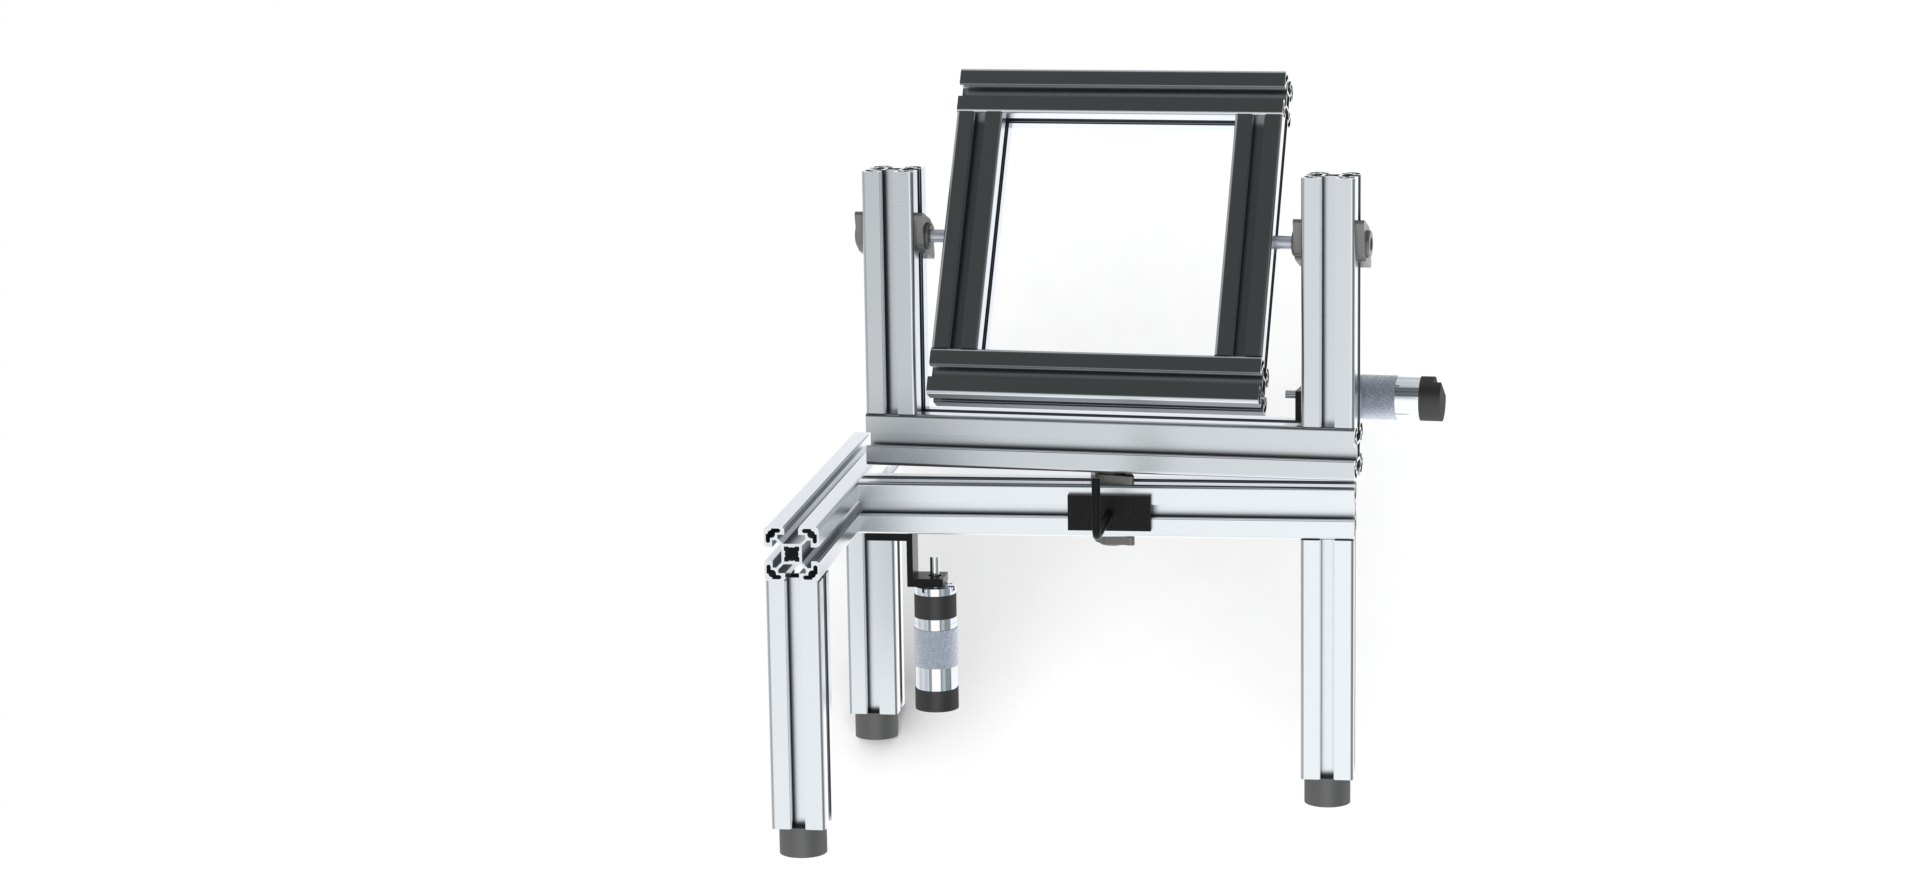
\includegraphics[width=1
\textwidth]{Sections/Miscellaneous/Images/FrontPagePicture.JPG}
\end{figure}


\textsc{Semester Project PRO4}\\[0.4cm]

\textsc{\large 4\textsuperscript{th} Semester Robotics - 2019}\\[0.4cm]
\textsc{\large Group 04}\\[0.4cm]


% Title
\rule{\linewidth}{0.5mm}\\[0.3cm]
{ \LARGE \bfseries Control and Regulation of Robotic Systems \\[0.3cm]}
\rule{\linewidth}{0.5mm}\\[1.2cm]

% Authors and supervisor
\begin{table}[h]
\centering
\begin{tabular}{ccccc}
                       \cline{1-1}  \cline{3-3}  \cline{5-5} 
Christian Eberhardt &  & Jakob Grøftehauge   &  & Lars Pedersen       \\
chebe17@student.sdu.dk &  & jakra17@student.sdu.dk &  & larpe17@student.sdu.dk \\ 
                       &  &                        &  &                       \\ 
                       &  &                        &  &                        \\
                                              \cline{1-1} \cline{3-3}  \cline{5-5}
Mads Kuhlmann-Jørgensen          &  & Jakob Møller kaad &  & Peter Christiansen     \\
makuh17@student.sdu.dk &  &                jakaa17@student.sdu.dk     &  & pechr17@student.sdu.dk  \\  
                       &  &                        &  &                        \\ 
\end{tabular}
\end{table}



% \begin{table}[h]
% \centering
% \begin{tabular}{ccccc}
% Christian Eberhardt &  & Jakob Grøftehauge   &  & Lars Pedersen       \\
%                       &  &                        &  &                       \\ \cline{1-1} \cline{3-3} \cline{5-5} \\
% chebe17@student.sdu.dk &  & jakra17@student.sdu.dk &  & larpe17@student.sdu.dk \\ 
%                       &  &                        &  &                        \\
% Mads Alber Kuhlmann          &  &                        &  & Peter Christiansen     \\
%                       &  &                        &  &                        \\ \cline{1-1} \cline{5-5}\\
% makuh17@student.sdu.dk &  &                        &  & pechr17@student.sdu.dk  \\  
% \end{tabular}
% \end{table}




%\vfill

\textbf{Supervisor:} Agus Ismail Hasan \\ %\hspace{0.5 cm}
%
% Bottom of the page
\textbf{Handover Date:} 29-05-2019
\end{center}
\end{titlepage}
\newpage
\pagenumbering{Roman}
\rfoot{\thepage}
\subfile{Sections/Miscellaneous/Abstract}
\newpage
\rfoot{Page \thepage \hspace{1pt} of \pageref{LastPage}}
\setcounter{page}{2}
\pagenumbering{arabic}
\tableofcontents



\newpage
\setlength{\parskip}{10pt plus 1pt minus 1pt} %Afstand mellem afsnit!!
\section{Introduction}\label{sec:opening}
\subfile{Sections/Miscellaneous/Introduction.tex}

\section{Problem Description}\label{sec:ProblemDescription}
\subfile{Sections/Miscellaneous/ProblemDescription.tex}

\section{Analysis}\label{sec:Analysis}
\subfile{Sections/Miscellaneous/Analysis.tex}

\section{Delimitation}\label{sec:Delimination}
\subfile{Sections/Miscellaneous/Delimitation.tex}

\section{Requirement Specifications}\label{sec:Requirements}
\subfile{Sections/Miscellaneous/Requirements.tex}

\section{System Analysis and Modelling}\label{sec:System_Modeling}
\subfile{Sections/System_Modelling/Modelling_of_Motor.tex}

\section{Control System Design}\label{sec:System_Design}
\subfile{Sections/System_Design/system_design.tex}
\section{System Integration and Implementation}\label{sec:System_Integration_N_Implementation}
\subfile{Sections/System_Implementation/Sys_Impl_FPGA.tex}
\subfile{Sections/System_Implementation/Sys_Impl_MicroC.tex}

\section{Tests}\label{sec:Test}
\subfile{Sections/Test/Test.tex}

\section{Discussion}\label{sec:Discussion}
\subfile{Sections/Miscellaneous/Discussion.tex}


\section{Conclusion}\label{sec:Conclusion}
\subfile{Sections/Miscellaneous/Conclusion.tex}
\newpage

\bibliographystyle{abbrv}
\bibliography{Bibliography}
 
\newpage

\section{Overview of digital Appendix}\label{sec:digital_appendix}
\subfile{Sections/Miscellaneous/digital_overview_appendix.tex}

\newpage
\section{Word list}\label{sec:wordlist}
\subfile{Sections/Miscellaneous/WordList.tex}




\end{document}
